\documentclass[12pt, a4paper]{article}

\usepackage [utf8]{inputenc}
\usepackage [IL2]{fontenc}
\usepackage [czech]{babel}
\usepackage{graphicx}
\usepackage[numbib]{tocbibind}
\usepackage{subcaption}
%\usepackage{hyperref}
\usepackage{float}
\graphicspath{{obrazky/}}
\newcommand{\Break}{\State \textbf{break} }

\setlength{\parindent}{0pt}

\usepackage{relsize}

%reference
\usepackage{hyperref}
\usepackage{url}

\hypersetup{
colorlinks=true,
linkcolor=black,
urlcolor=blue,
pdftitle={Overleaf Example},
pdfpagemode=FullScreen,
}

\title{
\includegraphics[width=10cm]{FAV_cmyk}

{\huge Semestrální práce z KIV/TI}

\vspace{0.5cm}
{\LARGE Logické řízení - sanitace nádrží}
\vspace{1cm} 

\Large Lukáš Runt (A20B0226P)

\large {\itshape lrunt@students.zcu.cz}

\vspace{0.1cm}
\Large Miroslav Vdoviak (A20B0268P)

\large \itshape{miravdov@students.zcu.cz}
}
\date{\vspace{6cm} \today}

\begin{document}

\begin{titlepage}
\clearpage\maketitle
\thispagestyle{empty}
\end{titlepage}

\tableofcontents

\section{Zadání}
\begin{figure}[H]
    \centering
    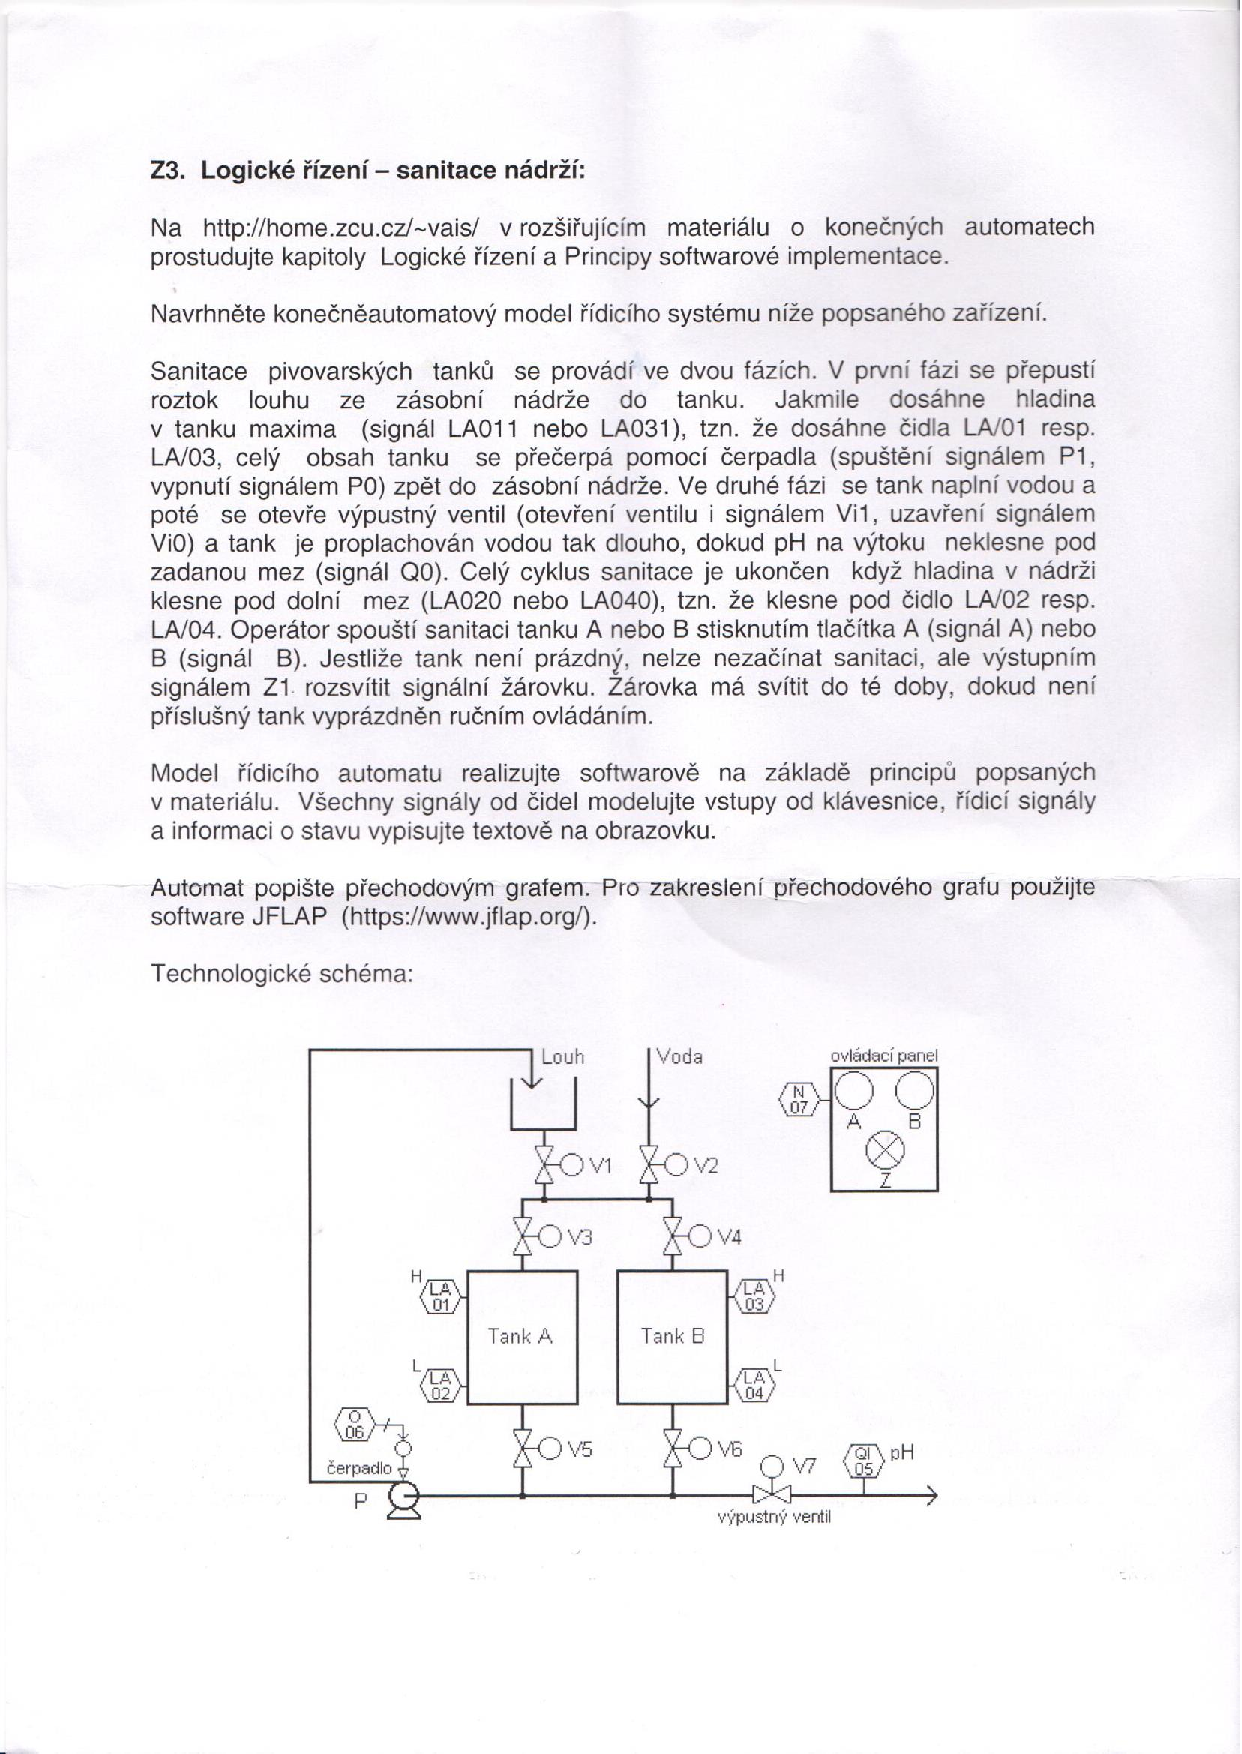
\includegraphics[width=13cm]{TI.pdf}
    \caption{Zadání}
    \label{obr1: Zadání}
\end{figure}
%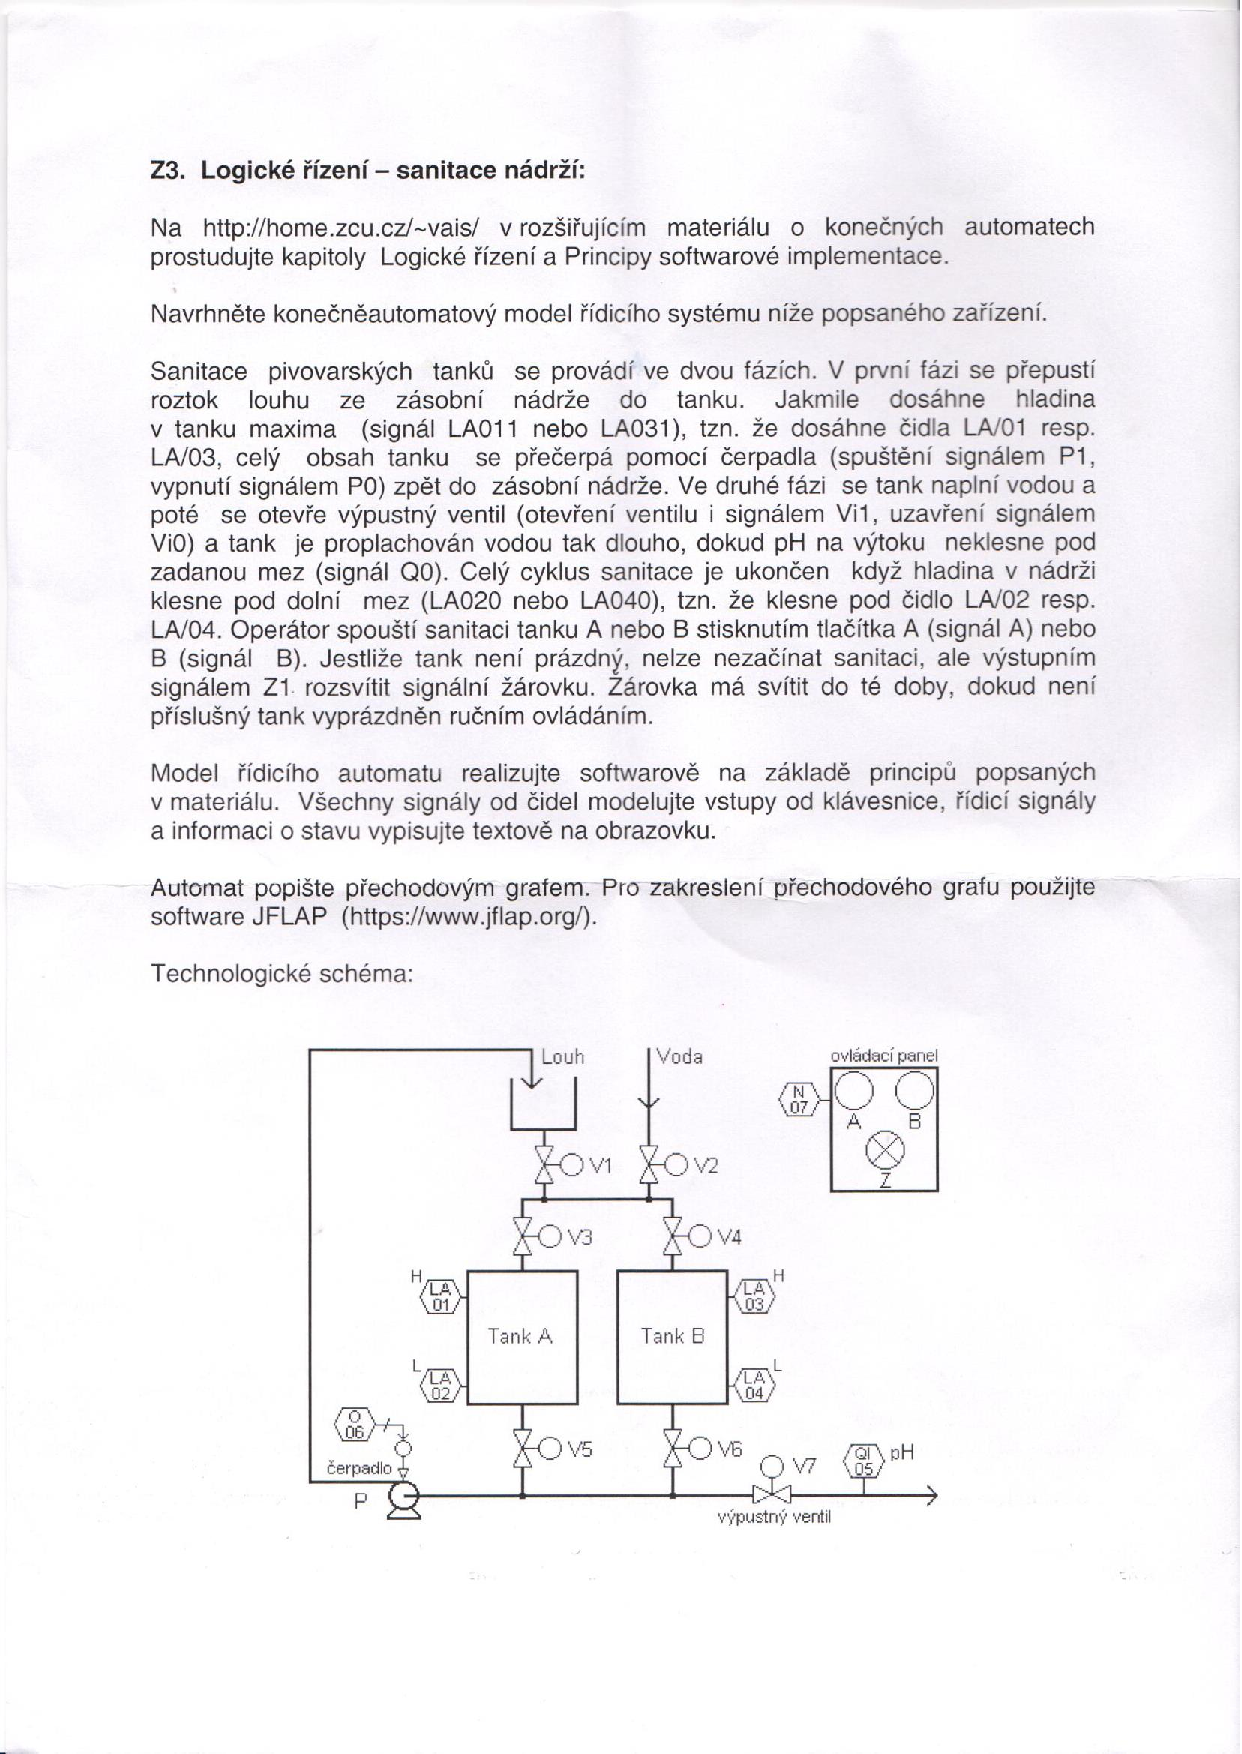
\includegraphics[width=14cm]{TI.pdf}

\section{Analýza úlohy}
\subsection{Konečný automat}
\subsubsection{Definice}

\noindent Definice konečného automatu
\[
    \mathlarger{A = (Q, \Sigma, \delta , q_0, F)} 
\]

\noindent$Q$ - konečná neprázdná množina stavů \newline
$\Sigma$ - konečná neprázdná množina vstupních symbolů \newline
$\delta$ - $Q \times \Sigma \rightarrow $ přechodová funkce \newline
$q_0 \in Q $ - počáteční stav \newline
$F\subseteq Q $ - množina koncových stavů \newline

Konečný automat je teoretický výpočetní model používaný v informatice pro studium formálních jazyků. Jedná se o počítač s konečným počtem stavů.
Automat postupně čte symboly, které přicházejí ze vstupu a následně pomocí nich přechází mezi jednotlivými stavy. Počet stavů je konečný. Tento jednoduchý počítač nemá žádnou paměť a jediné,
co si pamatuje je aktuální stav. V praxi se používá pro vyhodnocování regulárních výrazů.

\begin{figure}[h!]
    \centering
    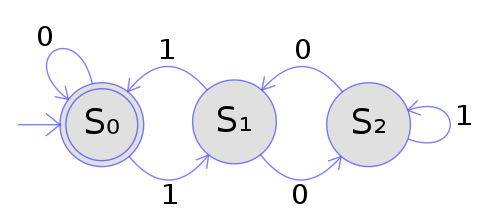
\includegraphics[width=8cm]{konecny_automat.png}
    \caption{Příklad konečného automatu se třemi stavy}
    \label{konecny_automat: 1}
\end{figure}

\subsubsection{Analýza}

Automat, který budeme vytvářet by měl obsahovat
\begin{itemize}
    \item 10 stavů (\hyperref[sec: stavy]{viz. stavy})
    \item 8 snímačů (\hyperref[sec: snimace]{viz. snímače})
    \item 6 řídících signálů (\hyperref[sec: signaly]{viz. signály})
    \item 2 spouštěcí tlačítka a kontrolní žárovku (\hyperref[sec: operator]{viz. řízení operátora})
\end{itemize}

Konečný automat budeme realizovat v programovacím jazyce \texttt{Java} a pro grafické rozhraní přichází v úvahu použití standardní knihovny
javy \texttt{java.swing a java.awt} nebo open source knihovny \texttt{JavaFX}. Uživatel bude ovládat aplikaci pomocí klávesnice. Při stisku tlačítka \texttt{A} by se měla spustit
sanitace tanku. Při dovršení maxima se spustí signál \texttt{LA011} a pomocí čerpadla \texttt{P} se nádrž vypustí
zpět do zásobní nádrže. V druhém kroku se tank napustí vodou a proplachuje se do té doby dokud \texttt{pH} výtoku neklesne pod dolní mez.
Obdobně by měl program fungovat i pro signál \texttt{B}. Pokud by uživatel chtěl zavolat sanitaci tanku, který není prázdný zobrazí se mu
chybové hlášení a měla by se rozsvítit žlutá chybová kontrolka. Grafické naplňování tanků je asi nejlepší naimplementovat
pomocí \texttt{timeru}, kdy se bude za krátký časový úsek měnit obraz. První variantou, jak toto uskutečnit, je pomocí vektorové grafiky, tedy bude se zvětšovat či zmenšovat o pár pixelů obdélník, který se bude vykreslovat uvnitř tanku
a tím se navodí iluze napouštění a vypouštění tanku, dále se budou měnit barevné kruhy které znázorňují spuštění/otevření zařízení. Druhou variantou je předpřipravit obrázky formátu \texttt{.gif}, které by se mohly měnit podle stavu modelu.

\section{Automatový model}

\subsection{Stavy}
Automat obsahuje následujících 10 stavů:

STAV 0 - Systém není v činnosti \newline 
STAV 1 - Tank A se napouští lihem \newline 
STAV 2 - Tanku A se přečerpává čerpadlem \newline 
STAV 3 - Tank A se plní vodou \newline 
STAV 4 - Tank A se proplachuje dokud není ph v normálu \newline 
STAV 5 - Tank A se vypouští \newline 
STAV 6 - Tank B se napouští lihem \newline 
STAV 7 - Tanku B se přečerpává čerpadlem \newline 
STAV 8 - Tank B se plní vodou \newline 
STAV 9 - Tank B se proplachuje dokud není ph v normálu \newline 
STAV 10 - Tank B se vypouští 

\newpage
\subsection{Přechodový graf}
Na následujícím obrázku je přechodový graf konečného automatu.
\begin{figure}[h]
\centering 
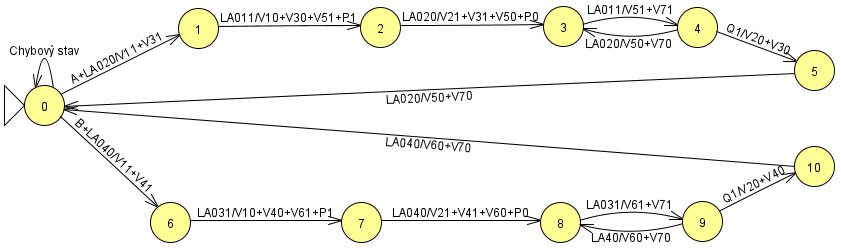
\includegraphics[width=14cm]{prechodovyAutomat}
\caption{Přechodový graf automatu}
\end{figure}

\subsection{Snímače}
Model automatu obsahuje následující signály od snímačů:
 
LA011 - Hladina překročila úroveň maxima tanku A \newline 
LA010 - Hladina klesla pod úroveň maxima tanku A \newline 
LA021 - Hladina překročila úroveň minima tanku A \newline 
LA020 - Hladina klesla pod úroveň minima tanku A \newline 
LA031 - Hladina překročila úroveň maxima tanku B \newline
LA030 - Hladina klesla pod úroveň maxima tanku B \newline 
LA041 - Hladina překročila úroveň minima tanku B \newline 
LA040 - Hladina klesla pod úroveň minima tanku B

\subsection{Řídící signály}
Model automatu obsahuje následující řídící signály:

P0 - Vypínám čerpadlo \newline 
P1 - Zapínám čerpadlo \newline 
Vi0 - Zavírám ventil \newline 
Vi1 - Otevírám ventil \newline 
Q0 - Ph se dostalo nad požadovanou mez \newline 
Q1 - Ph se dostalo pod požadovanou mez 

\newpage
\subsection{Řízení operátora}
Panel operátora obsahuje následující položky:

A - Sanitace tanku A \newline 
B - Sanitace tanku B \newline 
Z - Žárovka

\subsection{Chybové stavy} \label{chyba}
\begin{itemize}
  \item Uživatel chce začít sanitarizaci tanku, který není prázdný
  \item Uživatel chce začít sanitarizaci tanku v době, kdy se sanitarizuje jiný tank
  \item Uživatel chce míchat líh s vodou
  \item Uživatel chce vylévat líh do potrubí
  \item Uživatel chce čerpat vodu do nádrže s lihem
\end{itemize}

\section{Implementace}
Program je implementován v jazyce Java. Při vytváření programu bylo zvažováno, zda nebudou nakresleny obrázky v nějakém z grafických editorů, které se budou postupně měnit. Toto nám, ale přišlo krajně nepraktické, a proto byla zvolena implementace s pomocí knihovny \texttt{Java Swing} a vektorovou grafikou, která se bude překreslovat podle aktuálního stavu. 

\vspace{0.25cm}
Tato knihovna vytváří okno v metodě \texttt{main()}, které má pevně stanovenou velikost. O obsah okna se stará třída \texttt{DrawingPanel}, která je zodpovědná o vzhled modelu. Tato třída obsahuje i logiku automatu. Při spuštění se vše inicializuje tak, aby se vykreslil automat ve stavu 0, tedy v nečinnosti.

\vspace{0.25cm}
Každá komponenta má svoji proměnnou, která uchovává její stav. Tento stav se poté promítá do výsledného grafického výstupu. Stavy komponent jsou reprezentovány barvami. Zelená znamená logickou 1 a červená logickou 0. Toto neplatí u žárovky, která je při logické 1 žlutá a při logické 0 šedá. Komponenta tanku je pak řešena tak, že uchovává data o její plnosti v procentech a druh jejího obsahu (voda, líh, vzduch), který je řešen pomocí enumu \texttt{Napln}. Stav označený zeleně v přechodovém grafu značí aktuální stav. Ostatiní stavy mají bílou barvu.

\vspace{0.25cm}
Stavy modelu jsou realizovány pomocí proměnné \texttt{stav} datového typu \texttt{Integer}. Do dalšího stavu, se dostaneme pomocí snímačů, které jsou simulovány uživatelem. Zde uživatel ovládá snímače manuálně pomocí klávesnice, tedy do dalších stavů se přechází jen pomocí uživatelova činu. Po zmáčknutí klávesy se spouští metoda \texttt{zjistiStavManual()}, která zjistí stav a podle toho spustí příšlušnou metodu \texttt{stav[1|2|3|4|5|6|7|8|9|10]}, která rozhodne jestli přišel pulz ze snímače, kterým se přechází do dalšího stavu a následně provádí případné změny modelu.  

\vspace{0.25cm}
Reakce na uživatele je vyřešena pomocí metody \texttt{keyListener()}, rozeznávající, která klávesa byla stisknuta nebo uvolněna. Díky této metodě lze spouštět jednotlivé sanitace a manuálně ovládat model, avšak manuální ovládání je povoleno jen, když je konečný automat ve stavu 0. K zjištění, zda je ovládání povoleno slouží metoda \texttt{isManualniPovoleno()}. Jestliže chce uživatel spustit akci, která nemůže být spuštěna z důvodu chybového stavu, je zavolána metoda \texttt{vypisChybu()}, která vypíše ve vyskakovacím okně chybu a rozsvítí žárovku, která zhasne po zavření okna, které se zobrazilo.

\section{Uživatelská příručka}

\subsection{Spuštění programu}
Aplikace se spouští pomocí příkazu v příkazové řádce. Před zadáním příkazu se musíme ujistit, zda se nacházíme ve stejné složce, jako jar soubor, který se chystáme spustit (\texttt{semestralkaTI.jar}). Aplikaci poté spustíme pomocí příkazu: \texttt{java -jar semestralkaTI.jar} \ref{spusteni}. Pro spuštění je předpokladem mít nainstalovanou Javu verze nejméně 11. Odkaz ke stažení Javy 11: \url{ https://www.oracle.com/java/technologies/downloads/#java11}

\begin{figure}[h]
\centering 
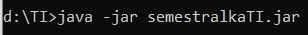
\includegraphics{prikladSpusteni}
\caption{Příklad spuštění}
\label{spusteni}
\end{figure}

Pokud se program podaří spustit zobrazí se model sanitarizace tanků s přechodovým grafem na pravé straně viz. obrázek \ref{vzhled}.

\begin{figure}[h]
\centering 
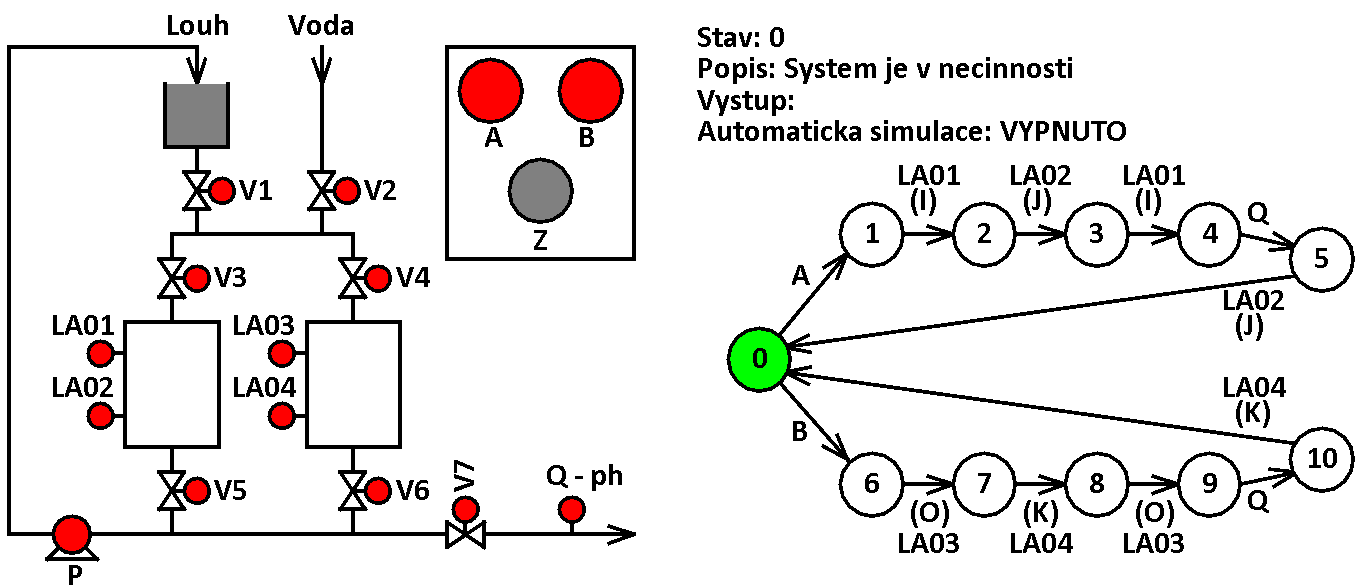
\includegraphics[width=14cm]{pospusteni}
\caption{Vzhled aplikace po spuštění}
\label{vzhled}
\end{figure}

\begin{figure}[h]
\centering 
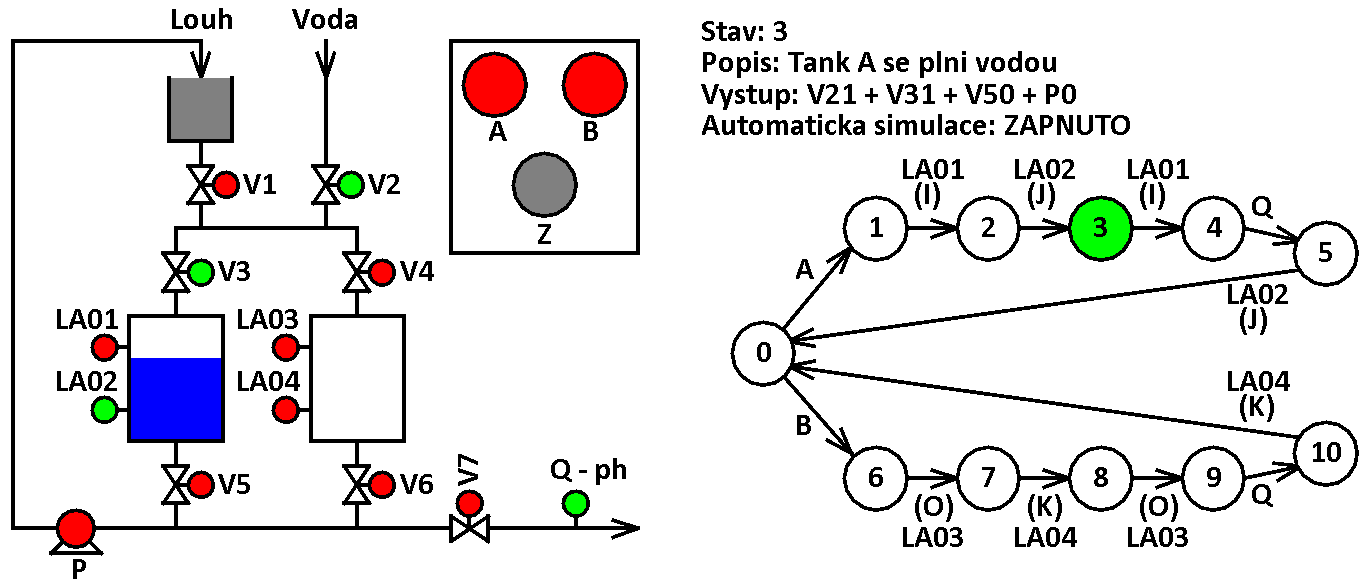
\includegraphics[width=14cm]{vprovozu}
\caption{Vzhled aplikace při provozu}
\end{figure}

\newpage
\subsection{Ovládání aplikace}
Po spuštění se zobrazí model ve stavu 0. Červená barva znamená logickou 0, tedy ventil je zavřený, tlačítko není stlačeno, ph není v požadované mezi, čerpadlo nečerpá líh, hladina v tanku není výš než snímač. Zelená barva znamená naopak logickou 1, tedy ventil je otevřený, tlačítko je stlačeno, atd. Žárovka má své barvy a to šedou pokud nesvítí a žlutou pokud svítí. Voda je znázorněna modrou barvou a líh barvou šedou.

\begin{figure}[h]
\centering
\begin{subfigure}{0.3\textwidth}
    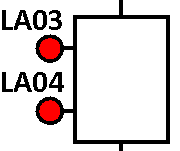
\includegraphics[width=\textwidth]{b}
    \caption{Prázdný tank}
\end{subfigure}
\hfill
\begin{subfigure}{0.3\textwidth}
    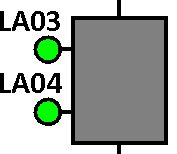
\includegraphics[width=\textwidth]{c}
    \caption{Tank plný lihu}
\end{subfigure}
\hfill
\begin{subfigure}{0.3\textwidth}
    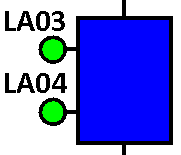
\includegraphics[width=\textwidth]{a}
    \caption{Tank plný vody}
\end{subfigure}
        
\caption{Vzhledy tanků při různé náplni}
\end{figure}

Aplikace se ovládá pomocí klávesnice. Uživatel má k dispozici ovládací panel (Spouštění sanitace nádrží) a manuální ovládání, které zahrnuje ovládání jednotlivých ventilů, snímačů a čerpadla. Při implementaci byla snaha o intuitivní ovládání, tedy ventily se ovládají pomocí jejich čísla, ostatní prvky se ovládají pomocí písmenka, kterým je daný prvek pojmenovaný. Snímače v tancích už bohužel moc intuitivní nejsou. Ovládají se pomocí kláves I, J, O, K. Pro přechod do dalšího stavu je potřeba aby uživatel zmáčkl klávesu příslušného snímače nebo tlačítka, tedy automat bude mezi stavy přecházet až po stisknutí správné klávesy. Podrobný výčet ovládání je uveden níže \ref{ovladani}. 

\begin{figure}[h]
\centering 
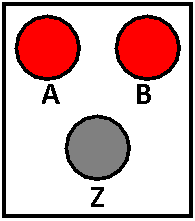
\includegraphics[width=4cm]{ovladacipanel}
\caption{Ovládací panel}
\end{figure}
\newpage

Pro sledování v jakém stavu se automat nachází je připravena pravá strana s přechodovým grafem. Nad přechodovým grafem zobrazen písemně stav a popis stavu, ve kterém se automat nachází. Tento popis se mění podle stavu automatu.

\begin{figure}[h]
\centering 
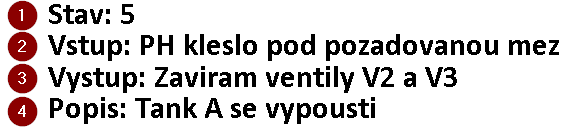
\includegraphics[width=14cm]{pismo}
\caption{Výpis stavu automatu}
\end{figure}

\begin{enumerate}
  \item Stav, ve kterém se automat nachází
  \item Vstup, který přiměl ke změnu stavu
  \item Výstupní signály od snímače (resp. operátora), který vyvolal předchozí přechod
  \item Popis děje, který se děje v tomto stavu
\end{enumerate}

Pod tímto měnícím se textem je vykreslen přechodový graf, který značí ve kterém stavu se automat nachází. Tento stav je zvýrazněn zeleně. U šipek přechodů je napsáno co příslušný přechod vyvolává, v závorce je pak klávesa, kterou se dá daný snímač ovládat.

\begin{figure}[h!]
\centering 
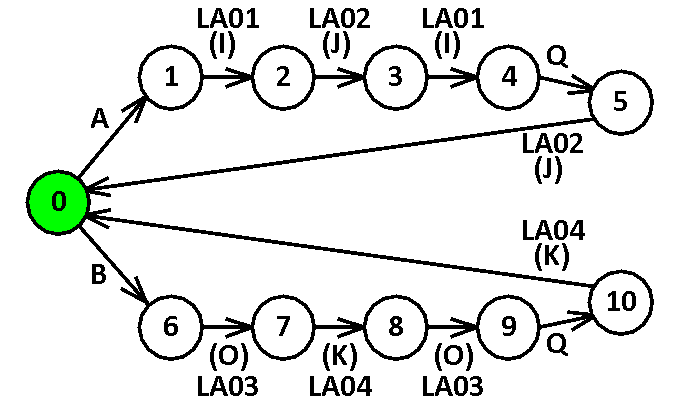
\includegraphics[width=8cm]{pa}
\caption{Přechodový graf v aplikaci}
\end{figure}    

Aplikace počítá s neobvyklým zacházením. Jsou tedy ošetřeny stavy, při kterých by mohlo dojít k chybě. Při chybovém stavu vyskočí na uživatele upozornění a v modelu se rozsvítí žárovka. Výčet chybových stavů lze najít zde: \ref{chyba}

\begin{figure}[h!]
\centering 
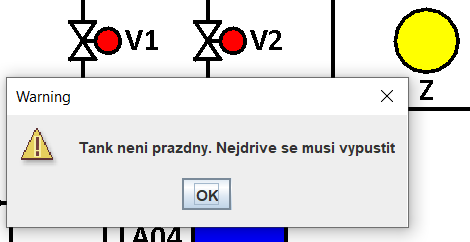
\includegraphics[width=9cm]{chyba}
\caption{Ukázka chybového stavu}
\end{figure}

\subsubsection{Výčet ovládacích kláves} \label{ovladani}
A - Spuštění sanitace tanku A \newline 
B - Spuštění sanitace tanku B \newline 
P - Manuální spuštění čerpadla \newline
Q - Ovládání snímače ph \newline
S - Zapínání/Vypínání automatické simulace \newline
I - Ovládání horního snímače tanku \newline
J - Ovládání spodního snímače tanku \newline
O - Ovládání horního snímače tanku \newline
K - Ovládání spodního snímače tanku \newline   
1 - Manuální otevření ventilu 1 \newline 
2 - Manuální otevření ventilu 2 \newline 
3 - Manuální otevření ventilu 3 \newline 
4 - Manuální otevření ventilu 4 \newline 
5 - Manuální otevření ventilu 5 \newline 
6 - Manuální otevření ventilu 6 \newline 
7 - Manuální otevření ventilu 7 \newline  

\newpage
\section{Závěr}
Výsledkem semestrální práce je funkční program simulující konečněautomatový model řídícího systému sanitace pivovarských tanků. Na práci by šla udělat nějaká vylepšení, například umožnit uživateli měnit velikost okna, ovšem myslíme si, že výsledek naší práce vypadá celkem solidně. V rámci úlohy jsme si vyzkoušeli napsat konečný automat, což byl také cíl. Byl to pro nás zážitek, který nás studijně obohatil a posunul o krok blíže k praktickým aplikacím teoreticky získaných vědomostí. 

\nocite{wiki:Konecny_automat}

\listoffigures

\bibliography{references}
\bibliographystyle{ieeetran}
\end{document}